% Created 2023-02-06 lun 12:21
% Intended LaTeX compiler: pdflatex
\documentclass[openany, a4paper]{book}
\usepackage[utf8]{inputenc}
\usepackage[T1]{fontenc}
\usepackage{graphicx}
\usepackage{longtable}
\usepackage{wrapfig}
\usepackage{rotating}
\usepackage[normalem]{ulem}
\usepackage{amsmath}
\usepackage{amssymb}
\usepackage{capt-of}
\usepackage{hyperref}
\usepackage{amsmath,amssymb,amsthm,geometry,hyperref,paralist,svg,thmtools,tikz,tikz-cd}
\usepackage{mathtools}
\usepackage[capitalise,noabbrev]{cleveref}
\usepackage{mdframed} \usepackage{svg}
\usepackage{environ} \NewEnviron{abmn}{\marginnote{\BODY}}
\usepackage{url}
\usepackage{color}
\usepackage{listings,chngcntr}% http://ctan.org/pkg/listings
\usepackage{multicol}
\usepackage{url}
\usepackage{tabularx}
\usepackage{xspace}
\usepackage{courier}
\definecolor{amber}{rgb}{1.0, 0.49, 0.0}
\definecolor{x11gray}{rgb}{0.75, 0.75, 0.75}
\lstset{ basicstyle=\footnotesize\mdseries\ttfamily, mathescape=true, frame=Trbl, numbers=left, keywordstyle=\color{blue}, showstringspaces=false, commentstyle=\color{x11gray}, stringstyle=\color{amber}, breaklines=true}
\renewcommand{\lstlistingname}{Code}
\setcounter{tocdepth}{1}
\newtheoremstyle{break}{\topsep}{\topsep}{\itshape}{}{\bfseries}{}{\newline}{}
\theoremstyle{plain}
\newtheorem{theorem}{Theorem}
\newtheorem{corollary}[theorem]{Corollary}
\newtheorem{proposition}[theorem]{Proposition}
\newtheorem{definition}[theorem]{Definition}
\newtheorem{lemma}[theorem]{Lemma}
\newtheorem{affirmation}[theorem]{Affirmation}
\theoremstyle{definition}
\newtheorem{example}{Example}
\newtheorem{exmpl}{Example}
\newtheorem{exercise}{Exercise}
\theoremstyle{remark}
\newtheorem{note}{Note}
\newtheorem{remark}{Remark}
\usetikzlibrary{arrows,automata,positioning}
\NewEnviron{obs}{\begin{mdframed}\begin{remark} \BODY \end{remark}\end{mdframed}}
\NewEnviron{nota}{\begin{mdframed}\begin{note} \BODY \end{note}\end{mdframed}}
\renewcommand{\qedsymbol}{\textbf{\therefore}}
\NewEnviron{blk}{\begin{mdframed}\BODY\end{mdframed}}
\newcommand{\nimplies}{\;\not\nobreak\!\!\!\!\implies}
\AtBeginDocument{\renewcommand{\thelstlisting}{\thesection.\arabic{lstlisting}}}
\AtBeginDocument{\counterwithin{lstlisting}{section}}
\newcommand{\R}{{\sf \small Read}\xspace}
\newcommand{\W}{{\sf \small Write}\xspace}
\hyphenation{Reentrant-Read-Write-Lock Stamped-Lock}
\author{Miguel Angel Piña Avelino}
\date{\today}
\title{A Study Of Concurrent Data Structures With Relaxed Semantics}
\hypersetup{
 pdfauthor={Miguel Angel Piña Avelino},
 pdftitle={A Study Of Concurrent Data Structures With Relaxed Semantics},
 pdfkeywords={},
 pdfsubject={},
 pdfcreator={Emacs 28.2 (Org mode 9.5.5)},
 pdflang={Spanish}}
\begin{document}

\maketitle
\tableofcontents


\chapter{Introduction}
\label{sec:org7d6637c}

\section{About Concurrent Computing}
\label{sec:org62b4aa0}

What is concurrent computing? This is a good question. We should first talk
about single-core and multi-core processors manufactured by the computer
industry. After the second world war and until the 90's the general purpose
cpus were single-core. All processes were executed in a single-core, and the
operating systems simulated concurrency using schedulers and other
techniques. In 2001, IBM introduce the first multi-core processor
\cite{ibmIBM100Power}, it allows that two processors work together at a very
high bandwidth (for the epoch) with large on-chip memories and with
high-speed buses. Since then, the amount of cores in each processors has been
increasing. We must consider as well the Moore's law, loosely speaking, this
law tells us that each year more and more transistors are placed into the
same space (i.e. electronic components and circuits are reduced in size), but
their speed cannot be increased without overheating. Consequently, the
industry move to ``multi-core'' architectures. In this architecture multiple
processors communicate through shared memory (RAM, hardware caches),
permitting make computing more effectively using \emph{parallelism}, where the
processors work together on a single task \cite{DBLP_books_daglib_0020056}.

\subsection{Classic concurrent computing}
\label{sec:org7c7fd0b}

\begin{itemize}
\item[{$\square$}] Basic Definitions
\item[{$\square$}] FLP impossibility result
\item[{$\square$}] Asynchronous Shared Memory
\item[{$\square$}] Primitive Synchronization Operations and Consensus
\end{itemize}

\subsection{Relaxed concurrent computing}
\label{sec:org91e2490}

\begin{itemize}
\item[{$\square$}] Relaxing the problem
\item[{$\square$}] Multiplicity preliminaries
\item[{$\square$}] Another relaxations?
\end{itemize}

\subsection{Work-stealing}
\label{sec:org05d3929}

\begin{itemize}
\item[{$\square$}] How it works the work-stealing
\item[{$\square$}] Classic algorithms
\item[{$\square$}] Idempotent algorithms
\item[{$\square$}] Work-stealing with multiplicity
\end{itemize}

\subsection{Data-Structures}
\label{sec:org02d4e9c}

\begin{itemize}
\item[{$\square$}] Queues with multiplicity
\item[{$\square$}]
\end{itemize}

\subsection{Contributions}
\label{sec:org0570d1d}

\subsection{Organization}
\label{sec:org9d691f4}


\section{Classic Concurrent Computing}
\label{sec:org5cee39c}

\section{Relaxed Concurrent Computing}
\label{sec:orga9439ba}




\chapter{Preliminaries}
\label{sec:org7471195}


\subsection{Mathematical model}
\label{sec:org42a5ccb}


\subsection{Realistic model of computation}
\label{sec:orge2a5bfb}

We consider a standard concurrent shared memory system with \(n \ge 2\)
\emph{asynchronous} processes, \(p_0, \ldots, p_{n-1}\), which may crash at any time
during an execution. The processes communicate with each other by invoking
atomic instructions of base objects: either simple Read/Write instructions to
\textbf{atomic objects}, or more powerful \textbf{Read-Modify-Write} instructions, such as
\texttt{Test-And-Set}, \texttt{Swap} or \texttt{Compare-And-Set}.

For simplicity we assume a single multicore chip where the processes run. In
our system we consider a memory hierarchy, where we have the following
elements in the hierarchy:

\begin{itemize}
\item Cache memory
\item Memory bus
\item Main memory
\end{itemize}

In this model, each processor core may read and
write to a single shared memory space. Usually each processor core has a
cache to operate with data from the shared memory. Often, this data is
transferred through a memory bus, allowing connect the processors with the
memory. The figure \ref{fig:arch} shows a simplified view of this model. In
the sections: \hyperref[sec:org12e37bc]{Cache memory}, \hyperref[sec:org90b8344]{Memory bus} and \hyperref[sec:orgad92fc2]{Main memory}, we explain more in
detail the meaning of each bullet of the list.

\begin{figure}
\begin{minipage}{\linewidth}
  \includesvg[width=\linewidth]{figs/architecture}
\end{minipage}
\caption{Simplified view of a modern computer system cache architecture}
\label{fig:arch}
\end{figure}


\subsection{Cache memory}
\label{sec:org12e37bc}

The cache memory is a special very high-speed memory that is very close to
the processor and the processes can access it very fast. The caches are used
to reduce average latencies to access storage structures
\cite{DBLP_series_synthesis_2020Nagarajan}. In recent multicore chips, the
cache memory is divided in three levels, two private levels (L1 and L2) for
each processor and a third level (L3) that is shared by the cores. The
purpose of the first two levels is to provide fast access to data and
instructions for the processors.

Each processor use the first level of cache to get the data and instructions
to execute them, usually the access to this level of cache is very fast
respect to the access to other levels.  The second level is often more
capacious than first level and is used to store data and instructions that
are close to be executed. In the third level, this cache is shared by many
processors and is used as feeder for the L2 cache.

\subsection{Memory bus}
\label{sec:org90b8344}

Is a computer bus that allows transfer data from the primary memory to the
CPU and the cache memory. It is made up of two parts: the data bus and the
address bus. The data bus is in charge of transfer information between the
primary memory and the correspondent chipset.
The address bus is used to retrieve information about the location of stored
information.


\subsection{Main memory}
\label{sec:orgad92fc2}

Is the responsible of hold the data that CPU need to access frequently, such
as instructions or data currently being processed. The CPU can access to
this information faster than the access to secondary memory.

\subsection{Consistency Memory Model and Cache Coherence}
\label{sec:orgb568483}

\begin{enumerate}
\item Consistency memory model
\label{sec:orge350402}

Following the simplified view of the cache architecture, we want to have a
correct shared memory. And what this means? The correctness of the shared
memory can be separated into two sub-issues: \emph{consistency} and \emph{correctness}.

The consistency (definitions) provide rules about loads and stores (memory
reads and writes) and how they act upon memory. These definitions must take
into account the behaviour of those operations on memory through access of
multiple threads or even a single thread. The consistency models define
correct shared memory behavior in terms of loads and stores, without
reference to caches or coherence \cite{DBLP_series_synthesis_2020Nagarajan}.
Shared memory correctness is specified by a memory consistency model (or
memory model). This specifies the allowed behavior of multithreaded programs
executing with shared memory.

The most intuitive and strongest memory model is the \emph{Sequential Consistency}
(SC). Another memory model used by systems \emph{x86} and \emph{SPARC} is \emph{Total Store Order}
(TSO), motivated by the desire of use \emph{first-in-first-out} write buffers to
hold the results of committed stores before writing results to the caches.
Additional to the prior memory model, "relaxed" or "weak" memory models are
considered, because these models shows that most memory orderings in strong
models are unnecessary \cite{DBLP_series_synthesis_2020Nagarajan}.

\item Cache coherence
\label{sec:org56f38c2}

Cache coherence protocols are used in response to solve a coherence problem
in cache. For example, a coherence problem can arise if multiple cores have
access to multiple copies of a datum, each one in a core, and at least one
them is a write access. The cache coherence protocols prevent the access to
stale data (incoherent data); this can be done using a set of rules
implemented by the distributed set of cores within a system. These
protocols use the common MOESI coherence states: modified (M), owned (O),
exclusive (E), shared (S) and invalid (I). The protocol acts like a state
machine, moving from one state to another based on the conditions of the
data and the cache memory \cite{DBLP_series_synthesis_2020Nagarajan}.
\end{enumerate}



\subsection{Memory fences}
\label{sec:org63671c4}

A memory fence is a barrier instruction that causes a CPU or compiler to
enforce a an ordering constraint on memory operations (loads and stores)
issued before and after the barrier instruction.

These instructions are necessary because most modern CPUs or compilers
employ performance optimizations, changing the order of the instructions on
one program, that could result in out-of-order execution. Normally these
optimizations are unnoticed in a single thread program, but can cause an
unpredictable behavior in concurrent programs.

For example, consider the following multi-thread program, with 2
threads, each one running in one core in a concurrent way:

Thread 1, core 1
\lstset{language=c++,label= ,caption= ,captionpos=b,numbers=none}
\begin{lstlisting}
while (z == 0);
print(y);
\end{lstlisting}

Thread 2, core 2
\lstset{language=c++,label= ,caption= ,captionpos=b,numbers=none}
\begin{lstlisting}
y = 30;
z = 1;
\end{lstlisting}

In this case, we might expect that the \texttt{print(y)} always print the number 30,
nevertheless, the compiler or the CPU could change the order of the
instructions for the thread 2, giving as result an execution where the value
for \texttt{y} is undefined and the instructions could be interleaved as follows:

\lstset{language=c++,label= ,caption= ,captionpos=b,numbers=none}
\begin{lstlisting}
z = 1; // Thread 2
while (z == 0); // Thread 1
print(y); // Thread 1
y = 30; // Thread 2
\end{lstlisting}

This execution is sequentially consistent, but is an out-of-order
execution producing an undefined result. With the use of memory barriers, we
can ensure that instructions don't be reordered. For example, our code could
be rewrite as follows:

Thread 1, core 1.
\lstset{language=c++,label= ,caption= ,captionpos=b,numbers=none}
\begin{lstlisting}
while (z == 0);
fence()
print(y);
\end{lstlisting}

Thread 2, core 2.
\lstset{language=c++,label= ,caption= ,captionpos=b,numbers=none}
\begin{lstlisting}
y = 30;
fence();
z = 1;
\end{lstlisting}


Languages as \texttt{Java} or \texttt{C++} provide instructions to establish synchronization
and ordering constraints between threads without an atomic operation. These
instructions have semantics well defined for

In the case of Java, we have static methods of the class VarHandle
(\texttt{java.lang.invoke.VarHandle}) that are refered as memory fence methods which
helps to provide fine-grained control of memory ordering. These statics
methods are \cite{varHandleJdk92017}:

\begin{description}
\item[{fullFence}] Ensures that loads and stores before the fence will not be
reordered with loads and stores after the fence. This method has memory
ordering effects compatible with
\texttt{atomic\_thread\_fence(memory\_order\_seq\_cst)}.
\item[{acquireFence}] Ensures that loads before the fence will not be reordered
with loads and stores after the fence. This method has memory ordering
effects compatible with \texttt{atomic\_thread\_fence(memory\_order\_acquire)}.
\item[{releaseFence}] Ensures that loads and stores before the fence will not
be reordered with stores after the fence. This method has memory ordering
effects compatible with \texttt{atomic\_thread\_fence(memory\_order\_release)}.
\item[{loadLoadFence}] Ensures that loads before the fence will not be
reordered with loads after the fence.
\item[{storeStoreFence}] Ensures that stores before the fence will not be
reordered with stores after the fence.
\end{description}

For C++, we have the function
\texttt{std::atomic\_thread\_fence}\cite{threadFenceCpp2020}, which establishes
memory synchronization ordering of non-atomic and relaxed atomic access, as
instructed by order, without an associated atomic operation. The type of
synchronization that can handle are the following:

\begin{itemize}
\item Fence-atomic synchronization
\item Atomic-fence synchronization
\item Fence-Fence Synchronization
\end{itemize}

And using a memory order\cite{memoryOrderCpp2020}, it can specifies how
memory accesses, including regular, non atomic memory accesses, are to be
ordered around an atomic operation. In total are six orders, from the
relaxed memory order to the sequential consistent memory order. They are:
\texttt{memory\_order\_relaxed}, \texttt{memory\_order\_consume}, \texttt{memory\_order\_acquire},
\texttt{memory\_order\_acq\_rel} and \texttt{memory\_order\_seq\_cst}. A note about
\texttt{atomic\_thread\_fence} functions, is that on x86 (x86\textsubscript{64}), these functions
issue no CPU instructions and only affect compile time code, with exception
for \texttt{std::atomic\_thread\_fence(std::memory\_order::seq\_cst)}, which issue the
full memory fence instruction \texttt{MFENCE}. For other archict



\section{Work-Stealing}
\label{sec:org7032d8f}

We analyze the algorithms for work-stealing described in the article Fully
Read/Write Fence Free Work-Stealing With Multiplicity, also the algorithm
called "Idempotent FIFO Work-Stealing", this because the algorithm have a
similar semantic than the prior algorithms.

\begin{figure}
\begin{minipage}{\linewidth}
  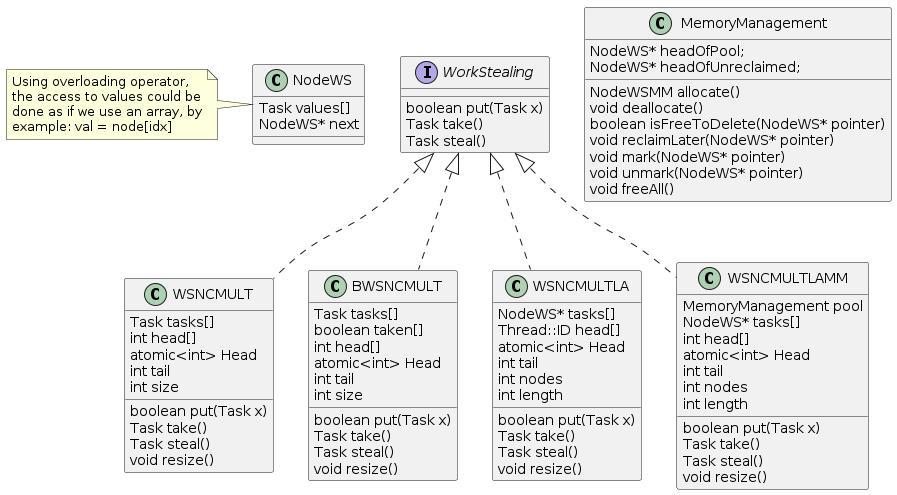
\includegraphics[width=\linewidth]{figs/objects.png}
\end{minipage}
\caption{Class Diagrama}
\label{fig:class_diagram}
\end{figure}


\subsection{Model}
\label{sec:org0c21abb}

\subsection{Known algorithms}
\label{sec:org4caeb29}

\subsection{Pseudocode for Work-Stealing with Weak Multiplicity}
\label{sec:org15543fc}



\section{Data-Structures}
\label{sec:orgd01690d}

\subsection{Queues}
\label{sec:org931c8a3}

\subsection{Stacks}
\label{sec:orgb62d6d6}


\section{Some Hardware Foundations}
\label{sec:org7b00bdf}

\subsection{Cache memory}
\label{sec:org259fb84}

The cache memory

\begin{enumerate}
\item Multiple caches
\label{sec:org86b0fa4}


\item Cache coherence protocols
\label{sec:orgb59a235}



\begin{enumerate}
\item MESI
\label{sec:orgf1d207a}


\item MOESI
\label{sec:org8780c37}
\end{enumerate}


\item Store Buffers
\label{sec:orga851279}
\end{enumerate}


\subsection{Reordering (CPU or Compiler)}
\label{sec:org0ed4a81}


\subsection{Memory Barriers}
\label{sec:orgdb4a426}


\begin{enumerate}
\item X86 and TSO architectures
\label{sec:org514df84}


\item Memory Fences
\label{sec:orgcd9933e}
\end{enumerate}


\subsection{Read-Modify-Write Operations}
\label{sec:orgd4318a6}


\subsection{Bibliography}
\label{sec:org958e680}

\begin{itemize}
\item \url{https://blog.the-pans.com/std-atomic-from-bottom-up/}
\end{itemize}


\subsection{Memory management}
\label{sec:org1260e75}

To implement efficiently the idempotent algorithms in an enviroment without
garbage collection, it's necessary use some technique or metodology to
provide garbage collection when atomic pointers are used or when distinct
threads want to reclaim the memory of the object associated to the pointer.

\begin{enumerate}
\item Strategies to delete shared pointers
\label{sec:org64fd8d2}

\begin{itemize}
\item Add pointers to list to safety delete.
\item Do this when there aren't more threads accessing to methods.
\begin{itemize}
\item Increase the counter when a thread enter to the method and decrease when
it exits.
\item Delete all pointers when the counter be equal to zero.
\end{itemize}
\end{itemize}


\item Hazard pointers
\label{sec:orgc4bc9f0}

The \emph{Hazard Pointers} is a technique to manage memory in languages where there
are not a garbage collector. This technique was proposed by Maged
Michael \cite{DBLP_journals_tpds_Michael04}. They are so called because
deleting a pointer that might be referenced by other thread(s) is
dangerous. If another threads keep holding references to that pointer and
proceed to access to that pointer after be deleted, you have a undefined
behavior \cite{DBLP_journals_tpds_Michael04}.

The basic idea of this technique is the following:

\begin{itemize}
\item If a thread want to use a pointer that another thread might want to
delete, it first sets a hazard pointer to the pointer, informing to the
other thread that deleting the pointer would be dangerous. Once the object
is not longer needed, the hazard pointer is cleared.
\item When a thread wants to delete the pointer, it must check if the hazard
pointers belonging to the other threads in the system. If no one has a
reference to the pointer, then, it's safe to delete the
pointer. Otherwise, it must be left until later.
\item Periodically, we must check the list of objects that have been left until
later to see if any of them can be deleted now.
\end{itemize}

A general pseudocode for this technique could be the following:

\lstset{language=c++,label= ,caption= ,captionpos=b,numbers=none}
\begin{lstlisting}
void func() {
    std::atomic<void*>& hp = get_hazard_pointer_for_current_thread();
    void* old_data = data.load();
    do {
        void* temp;
        do{ // Loop until you've set the hazard pointer
            temp = old_data;
            hp.store(old_data);
            old_data = data.load();
        } while (old_data != temp);
          }while (old_data &&
            !data.compare_exchange_strong(old_data, old_data->next);
    // Do something with old_data
    hp.store(nullptr); // clearing usage of hazard pointer
    // Trying clearing
    if (outstanding_hazard_pointers_for(old_head))
    {
        reclaim_later(old_data);
    }
    else
    {
        delete old_data;
    }
    delete_nodes_with_no_hazards();
}
\end{lstlisting}


\item Atomic Smart Pointers (Herlihy, Chapter 19) (Not available for GCC and CLang)
\label{sec:orgbcd15f1}


When a memory region is reclaimed, the programmer cannot know how that
region of memory will be reused or if even whether it is reused. We need a
way of developing a (general) solution to prevent the sorts of races
when a memory region is reclaimed by many threads asynchronously. We can to
do this by delaying reclamation.
Thinking in terms of pending operations on a concurrent data structure, a
sufficient condition is that \emph{memmory is only reclaimed when it is impossible
for any pending operation to access in the future}.

This property could be also achieved by \emph{reference counting}. In a reference
counted implementation of a data-structure (like a list), a counter of type
atomic<int> is associated with each node. Whenever a reference to node N is
created
\end{enumerate}


\section{Memory management for work-stealing algorithms}
\label{sec:orge078315}

It is well known that C++ does not have a garbage collector like Java. Since
the publish of the \href{https://en.cppreference.com/w/cpp/11}{Standard C++11}, new features for memory management were
added. For example, a concurrency support library and smart pointers. These
last are used to help ensure that programs are free of memory and resources
leaks and are exception safe.

For algorithms like Chaselev\cite{circular.work.stealing},
cilk\cite{implementation_cilk5}, Idempotent FIFO and Idempotent
LIFO\cite{maged.vechev.2009}, whose specification describe the use of simple
structures and variables, we can manage them using smart pointers to avoid
problems with memory management, but in the case of Idempotent
DEQUE\cite{maged.vechev.2009}, it need to use a more complex structure to
avoid problems like the \href{https://www.stroustrup.com/isorc2010.pdf}{ABA problem}.


\section{C++ Memory model}
\label{sec:org1c123b4}

\subsection{Memory model basics}
\label{sec:orgaccdc95}

\begin{enumerate}
\item Objects and memory locations
\label{sec:orga356001}


\item Objects, memory locations, and concurrency
\label{sec:org1aaf9a3}


\item Modification orders
\label{sec:org2eec728}
\end{enumerate}


\subsection{Atomic operations and types in C++}
\label{sec:org0bcdb11}


\begin{enumerate}
\item The standard atomic types
\label{sec:org12d65ef}

\item Operations on std::atomic\textsubscript{flag}
\label{sec:org202253b}

\item Operations on std::atomic<boolean>
\label{sec:org0ff3d70}

\item Operations on std::atomic<T*>: pointer arithmetic
\label{sec:orgc885c52}

\item Operations on standard atomic integral types
\label{sec:orgeb9b6c3}

\item The std::atomic<> primary class template
\label{sec:orgc369aaa}

\item Free functions for atomic operations
\label{sec:org27a7154}
\end{enumerate}

\subsection{Synchronizing operations and enforcing ordering}
\label{sec:orga51ca08}

\begin{enumerate}
\item The synchronization relationship
\label{sec:org8e0ff0d}

\item The happens-before relationship
\label{sec:org30baa7e}

\item Memory ordering for atomic operations
\label{sec:orgdedcff1}

\item Release sequences and synchronizes-with
\label{sec:orga2858a7}

\item Fences
\label{sec:org8d90edf}

\item Ordering non-atomic operations with atomics
\label{sec:org85c712e}

\item Ordering non-atomic operations
\label{sec:orgd158665}
\end{enumerate}


\section{Guidelines for designing data-structures for concurrency}
\label{sec:org695e5c3}

\begin{itemize}
\item Ensure that no thread can see a state where the invariants of the
data-structure have been broken by the action of the another thread.

\item Take care to avoid race conditions inherent in the interface to the
data-structure by providing functions for complete operations rather than
for operations steps.

\item Pay attention to how the data-structure behaves in the presence of
exceptions to ensure that the invariants are not broken.

\item Minimize the opportunities for deadlock when using the data-structure by
restricting the scope of locks and avoiding nested locks where possible.
\end{itemize}





\chapter{Work Stealing}
\label{sec:orgd528155}

\chapter{Modular Basket Queues}
\label{sec:org6d7bfa6}

\chapter{Conclusions}
\label{sec:orgb5374c4}


\chapter{Bibliography}
\label{sec:org17d95f1}
\bibliographystyle{plainurl}
\bibliography{refs}
\end{document}